
\documentclass[ review  , 3p ]{elsarticle}
%default = preprint (single sapce), review = doublespace
%detail class option: https://www.elsevier.com/__data/assets/pdf_file/0008/56843/elsdoc-1.pdf

% eliminate "Preprinted to Elsevier"
\makeatletter
\def\ps@pprintTitle{%
 \let\@oddhead\@empty
 \let\@evenhead\@empty
 \def\@oddfoot{\centerline{\thepage}}%
 \let\@evenfoot\@oddfoot}
\makeatother

%%% Begin My package additions %%%%%%%%%%%%%%%%%%%
\usepackage[hyphens]{url}



\usepackage{lineno} % add
\providecommand{\tightlist}{%
  \setlength{\itemsep}{0pt}\setlength{\parskip}{0pt}}

\usepackage{graphicx}

\usepackage{zxjatype}
\usepackage{xeCJK}
\setCJKmainfont{ipaexm.ttf}
\setCJKsansfont{ipaexg.ttf}
\setCJKmonofont{ipaexg.ttf}

\usepackage{color}

\usepackage{booktabs}
\usepackage{longtable}
\usepackage{array}
\usepackage{multirow}
\usepackage{wrapfig}
\usepackage{float}
\usepackage{colortbl}
\usepackage{pdflscape}
\usepackage{tabu}
\usepackage{threeparttable}
\usepackage{threeparttablex}
\usepackage[normalem]{ulem}
\usepackage{makecell}
\usepackage{xcolor}


%\usepackage{xpatch}
%\xpatchcmd{\MaketitleBox}{\hrule}{}{}{}% remove first horizontal rule (above abstract)
%\xpatchcmd{\MaketitleBox}{\hrule}{}{}{}% remoce second horizonral rule (below keywords)
%%%%%%%%%%%%%%%% end my additions to header

\usepackage[T1]{fontenc}
\usepackage{lmodern}
\usepackage{amssymb,amsmath}
\usepackage{ifxetex,ifluatex}
\usepackage{fixltx2e} % provides \textsubscript
% use upquote if available, for straight quotes in verbatim environments
\IfFileExists{upquote.sty}{\usepackage{upquote}}{}
\ifnum 0\ifxetex 1\fi\ifluatex 1\fi=0 % if pdftex
  \usepackage[utf8]{inputenc}
\else % if luatex or xelatex
  \usepackage{fontspec}
  \ifxetex
    \usepackage{xltxtra,xunicode}
  \fi
  \defaultfontfeatures{Mapping=tex-text,Scale=MatchLowercase}
  \newcommand{\euro}{€}
\fi
% use microtype if available
\IfFileExists{microtype.sty}{\usepackage{microtype}}{}
\bibliographystyle{elsarticle-harvard}
\usepackage{tabularx}
\ifxetex
  \usepackage[setpagesize=false, % page size defined by xetex
              unicode=false, % unicode breaks when used with xetex
              xetex]{hyperref}
\else
  \usepackage[unicode=true]{hyperref}
\fi
\hypersetup{breaklinks=true,
            bookmarks=true,
            pdfauthor={},
            pdftitle={Short Paper},
            colorlinks=false,
            urlcolor=blue,
            linkcolor=magenta,
            pdfborder={0 0 0}}
\urlstyle{same}  % don't use monospace font for urls

\setcounter{secnumdepth}{5}

\newlength{\cslhangindent}
\setlength{\cslhangindent}{1.5em}
\newlength{\csllabelwidth}
\setlength{\csllabelwidth}{3em}
\newenvironment{CSLReferences}[3] % #1 hanging-ident, #2 entry spacing
 {% don't indent paragraphs
  \setlength{\parindent}{0pt}
  % turn on hanging indent if param 1 is 1
  \ifodd #1 \everypar{\setlength{\hangindent}{\cslhangindent}}\ignorespaces\fi
  % set entry spacing
  \ifnum #2 > 0
  \setlength{\parskip}{#2\baselineskip}
  \fi
 }%
 {}
\usepackage{calc} % for \widthof, \maxof
\newcommand{\CSLBlock}[1]{#1\hfill\break}
\newcommand{\CSLLeftMargin}[1]{\parbox[t]{\maxof{\widthof{#1}}{\csllabelwidth}}{#1}}
\newcommand{\CSLRightInline}[1]{\parbox[t]{\linewidth}{#1}}
\newcommand{\CSLIndent}[1]{\hspace{\cslhangindent}#1}

% Pandoc toggle for numbering sections (defaults to be off)


% Pandoc header


\begin{document}
  \begin{frontmatter}

    \title{Charitable Giving, Tax Reform, and Government Efficiency\tnoteref{1}}
            \tnotetext[1]{This research is base on}
                \author[Osaka University]{
      Hiroki Kato 
       \corref{*} }
     \ead{vge008kh@stundent.econ.osaka-u.ac.jp}   %to avoid auto-link, use \@ instead of @
        \author[Chiba University]{
      Tsuyoshi Goto 
      }
      %to avoid auto-link, use \@ instead of @
        \author[Kobe University]{
      Yong-Rok Kim 
      }
      %to avoid auto-link, use \@ instead of @
            \address[Osaka University]{Graduate School of Economics, Osaka University, Japan}
        \address[Chiba University]{Graduate School of Economics, Chiba University, Japan}
        \address[Kobe University]{Graduate School of Economics, Kobe University, Japan}
            \cortext[*]{Corresponding Author.}
      
        \begin{abstract}
      Brah
    \end{abstract}
      
        \begin{keyword}
      Charitable giving, Giving price, Tax reform, Governement efficiency, South Korea
       \JEL{D91, I10, I18} 
    \end{keyword}
    
  \end{frontmatter}

  \hypertarget{introduction}{%
  \section{Introduction}\label{introduction}}
  
  In many countries, governments set a tax relief for charitable giving. This is because, if subsidizing charitable giving induces a large increase in donations, it is desirable for public good provision. To evaluate the effect of tax relief, many papers investigate the elasticity of charitable donations with respect to their tax price (Almunia et al., 2020; Auten et al., 2002; Bakija and Heim, 2011; Fack and Landais, 2010; Randolph, n.d.). Focusing on the tax deduction or tax credit on the charity, they show that the price elasticity of giving is about -1 or more in terms of absolute value, which means that the tax relief for the charitable giving is good in the sense that 1\% tax relief derives more than 1\% donation.
  
  However, if the government can provide public good more efficiently than the direct donation, the donation may not be preferable because the public good provision via donation would be costly then.
  Moreover, when the government is much more efficient than charities, people may not donate so much even if they have a warm-glow preference. Saez (2004) suggests that the change of the relative price between public good provision by donation and government will change the behavior of people and the price elasticity of donation.
  However, the evaluation about the efficiency of the government is usually subjective and different for people. If someone regard the government as efficient, the perceived relative price of giving would be high for them. Thus, the giving behavior would be affected by the subjective perception towards the government.
  
  Considering these points, this paper investigates (1) the price elasticity of giving and (2) whether the different perception towards the government cause the different giving behavior using South Korean panel data.
  Our first main concern is the price elasticity of charity. South Korea (Korea hereafter) experienced the tax reform in 2014, from when the tax relief on charitable giving was conducted by tax credit, though tax deduction had been used before 2014. Thus, we exploit this tax reform as an exogenous policy change to derive the price elasticity of giving. Since the extant research focus on the tax reform within the scheme of tax deduction or tax credit, this paper firstly deals with the tax reform from tax deduction system to tax credit system.
  Our result classifies that the price elasticity of giving in Korea is -1.07 \textasciitilde{} -1.26, which is within the range of the extant research.
  
  Our second concern is the relationship between the giving behavior and the perception towards the government. As we explained, people feeling administrative inefficiency would consider the direct donation is more efficient and would have more willingness to donate. Using the Korean field data, we investigate this and show that the amount of donation is not different between those who regard government as inefficient and the others, though the giving price elasticity of the former is more elastic than the latter. This means that those who think of government as inefficient have more willingness to donate for 1\% reduction of giving price.
  
  This paper contributes two strands of charitable giving literature: the elasticity of charitable donations with respect to their tax price and the perception of government's inefficiency. The examples of papers in the first strand are (Almunia et al., 2020; Auten et al., 2002; Bakija and Heim, 2011; Fack and Landais, 2010; Randolph, n.d.). They typically use the tax return data, the main part of which is the data about wealthy people. Since our data is based on survey, which represents the income distribution of population, we believe that we can estimate the giving price elasticity of population more precisely. Using the data with low-income households may be difficult to estimate the giving price elasticity in terms of intensive margin since they are expected to donate less than high-income households. To address this issue, we estimate not only the elasticity of intensive margin, as most of papers do, but also the elasticity of extensive margin following Almunia et al. (2020).
  Moreover, we use the data of Korea, a non-Western country, which the extant research did not examine\footnote{This point may be important since @Kim2021 reports that the giving behavior is strongly affected by the cultural matter such as the religious belief.}.
  
  In the second strand, there are some experimental studies and papers considering the tax evasion. Using an experiment, Li et al. (2011) compare people's willingness to give money for private charities and government agencies both of whose missions are the same. They show that people tend to donate for private charities more than government agency though they do not directly investigate the relationship between people's perception toward the government and giving behavior. Sheremeta and Uler (2020) show that people increase the voluntary public good provision when they face the wasteful government spending in the experimental setting. Although the government in their setting does not provide public good, they suggest that the willingness for donation may increase if people perceive the inefficiency of government. In the tax evasion literature, several paper suggests the perceived inefficiency of government reduce tax morale (Anderson, 2017; Frey and Torgler, 2007; Hammar et al., 2009). We contribute on this literature by showing the relation between the perception of government efficiency and the giving behavior.
  
  This paper consist of XXX sections. Section 2 and 3 respectively explain the institutional background and data. Section 4 deals with the analysis of giving price elasticity and section 5 shows the analysis of perceptions toward the government. We discuss the result in section 6 and section 7 concludes.
  
  \hypertarget{institutional-background}{%
  \section{Institutional background}\label{institutional-background}}
  
  In this section, we describe the income tax relief for charitable giving in Korea and used dataset.
  
  \hypertarget{tax-relief-for-charitable-giving-by-tax-deduction-and-tax-credit}{%
  \subsection{Tax relief for charitable giving by tax deduction and tax credit}\label{tax-relief-for-charitable-giving-by-tax-deduction-and-tax-credit}}
  
  In the South Korea, the tax policy about charitable giving drastically changed in 2014. Before then, tax relief of charitable giving was provided by tax deduction while, from 2014, tax relief by tax credit was introduced instead of tax deduction.
  
  The tax deduction and tax credit may have different effects on giving behavior. This subsection summarize the difference of tax deduction and tax credit.
  Consider that a household has a choice between private consumptions (\(x_i\)) and charitable giving (\(g_i\)). Let \(y_i\) be pre-tax total income.
  Then, the budget constraint is
  
  \[
      x_i + g_i = y_i - T_i(y_i, g_i).
  \]
  \(T_i\) is tax amount which depends on the pre-tax income and charitable giving.
  On one hand, tax deduction reduces taxable income by giving, that is,
  
  \[
      T_i = \tau(y_i - g_i) \cdot (y_i - g_i),
  \]
  
  where \(\tau(\cdot)\) is the marginal income tax rate which is determined by \(y_i - g_i\). The budget constraint will be
  
  \[
      x_i + [1 - \tau(y_i - g_i)]g_i = [1 - \tau(y_i - g_i)] y_i.
  \]
  
  Thus, the giving price compared to the price of private consumption is \(p_i^{d} \equiv 1 - \tau(y_i - g_i)\) in tax deduction system. Since the giving price in tax deduction scheme varies depending on (1) the income level and (2) the amount of charitable giving, it is endogenous to them, i.e. (1) and (2).
  
  On the other hand, tax credit reduces tax amount directly, that is,
  
  \[
      T_i = \tau(y_i)\cdot y_i - m g_i,
  \]
  
  where \(m \in [0, 1]\) is the tax credit rate. Under the tax credit system, the budget constraint is
  
  \[
      x_i + (1 - m) g_i = [1 - \tau(y_i)] y_i.
  \]
  
  Thus, the giving price of tax credit system will be \(p_i^c = 1 - m\), which is only dependent on the tax credit rate \(m\), which is exogenously determined by the government.
  Therefore, the giving price in the tax credit system would not be manipulated by donors.
  
  \hypertarget{korean-tax-reform-in-2014-need-modification-by-kim-san}{%
  \subsection{Korean tax reform in 2014 (Need modification by Kim san)}\label{korean-tax-reform-in-2014-need-modification-by-kim-san}}
  
  The tax incentives for charitable giving in Korea stared in 2000. Since the income tax deduction was initially used as a tax incentive and the marginal income tax rate was determined as Figure \ref{tab:tabTaxRate}, the minimum giving price before 2014 was 0.62. In addition, the government set the limit of charitable giving deduction, which was initially the 5\% of income. The government gradually expanded the limit and it finally became 30\% in 2012.
  
  \begin{table}
  
  \caption{\label{tab:tabTaxRate}Marginal Income Tax Rate}
  \centering
  \fontsize{8}{10}\selectfont
  \begin{threeparttable}
  \begin{tabular}[t]{lccccccc}
  \toprule
  Income/Year & 2008 & 2009 & 2010 \textasciitilde{} 2011 & 2012 \textasciitilde{} 2013 & 2014 \textasciitilde{} 2016 & 2017 & 2018\\
  \midrule
  (A) \textasciitilde{} 1200 & 8\% & 6\% & 6\% & 6\% & 6\% & 6\% & 6\%\\
  \cmidrule{1-8}
  (B) 1200 \textasciitilde{} 4600 & 17\% & 16\% & 15\% & 15\% & 15\% & 15\% & 15\%\\
  \cmidrule{1-8}
  (C) 4600 \textasciitilde{} 8800 & 26\% & 25\% & 24\% &  & 24\% & 24\% & 24\%\\
  \cmidrule{1-4}
  \cmidrule{6-8}
  (D) 8800 \textasciitilde{} 15000 &  &  &  & \multirow{-2}{*}{\centering\arraybackslash 24\%} & 35\% &  & 35\%\\
  \cmidrule{1-1}
  \cmidrule{5-6}
  \cmidrule{8-8}
  (E) 15000 \textasciitilde{} 30000 &  &  &  & 35\% &  & \multirow{-2}{*}{\centering\arraybackslash 35\%} & 38\%\\
  \cmidrule{1-1}
  \cmidrule{5-5}
  \cmidrule{7-8}
  (F) 30000 \textasciitilde{} 50000 &  &  &  &  &  & 38\% & 40\%\\
  \cmidrule{1-1}
  \cmidrule{7-8}
  (G) 50000 \textasciitilde{} & \multirow{-4}{*}{\centering\arraybackslash 35\%} & \multirow{-4}{*}{\centering\arraybackslash 35\%} & \multirow{-4}{*}{\centering\arraybackslash 35\%} & \multirow{-2}{*}{\centering\arraybackslash 38\%} & \multirow{-3}{*}{\centering\arraybackslash 38\%} & 40\% & 42\%\\
  \bottomrule
  \end{tabular}
  \begin{tablenotes}
  \item Notes: Marginal income tax rates applied from 2008 to 2018 are summarized. The income level is shown in terms of 10,000 KRW, which is approximately 10 United States dollars (USD) at an exchange rate of 1,000 KRW to one USD.
  \end{tablenotes}
  \end{threeparttable}
  \end{table}
  
  However, the government reformed tax system again in 2014, where the tax credit was introduced instead of tax deduction. Since then, 15\% of the total amount of charitable giving has been allowed as a tax credit, which means that the giving price from 2014 is 0.85 irrelevant to the income level.
  
  Summarizing this, compared to tax credit system, the high income household, whose (average) income tax rate is more than 15\%, get benefit from charitable giving under the tax deduction system. However, middle or low income households would enjoy tax relief in tax credit system more than tax deduction system. We exploit this policy change as an identification strategy.
  
  \textbf{Additional description needed:}
  
  \begin{itemize}
  \tightlist
  \item
    The limit of tax relief compared to income under the tax credit system (it was 30\% in tax deduction system in 2012).
  \item
    The reason why the government execute the tax reform (short background)
  \item
    Description of donation market in Korea (what \% of GDP is the donation market?/ what is the main outlet of the charity fund?)
  \item
    Political background
  \end{itemize}
  
  \hypertarget{data}{%
  \section{Data}\label{data}}
  
  \hypertarget{time-series-of-chariable-giving}{%
  \subsection{Time Series of Chariable Giving}\label{time-series-of-chariable-giving}}
  
  \begin{figure}
  
  {\centering 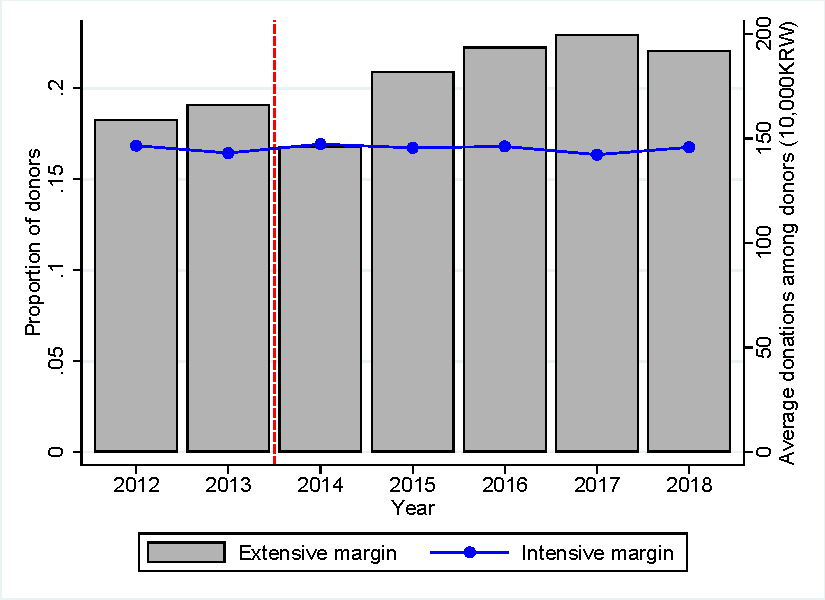
\includegraphics[width=0.9\linewidth]{C:/Users/vge00/Desktop/NaSTaB/_assets/SummaryOutcome} 
  
  }
  
  \caption{Proportion of Donors and Average Donations among Donors}\label{fig:unnamed-chunk-1}
  \end{figure}
  
  \hypertarget{summary-statistics}{%
  \subsection{Summary Statistics}\label{summary-statistics}}
  
  \begin{table}
  
  \caption{\label{tab:kableSummaryCovariate}Summary Statistics}
  \centering
  \fontsize{8}{10}\selectfont
  \begin{tabular}[t]{lcccccccc}
  \toprule
   & N & Mean & Std.Dev. & Min & p25 & p50 & p75 & Max\\
  \midrule
  \addlinespace[0.3em]
  \multicolumn{9}{l}{\textbf{Income and Giving Price}}\\
  \hspace{1em}Annual taxable income (unit: 10,000KRW) & 53269 & 1876.121 & 2700.965 & 0.00 & 0.00 & 900.00 & 2902.445 & 91772.00\\
  \hspace{1em}Giving Price & 62878 & 0.858 & 0.036 & 0.62 & 0.85 & 0.85 & 0.850 & 0.94\\
  \addlinespace[0.3em]
  \multicolumn{9}{l}{\textbf{Charitable Donations}}\\
  \hspace{1em}Annual charitable giving (unit: 10,000KRW) & 67849 & 29.522 & 132.914 & 0.00 & 0.00 & 0.00 & 0.000 & 10000.00\\
  \hspace{1em}dummy of Donation > 0 & 67849 & 0.203 & 0.402 & 0.00 & 0.00 & 0.00 & 0.000 & 1.00\\
  \addlinespace[0.3em]
  \multicolumn{9}{l}{\textbf{Government Efficiency}}\\
  \hspace{1em}Current Tax-Welfare Balance & 29272 & -0.137 & 0.889 & -2.00 & -1.00 & 0.00 & 0.000 & 2.00\\
  \hspace{1em}Ideal Tax-Welfare Balance & 29273 & 0.541 & 0.721 & -2.00 & 0.00 & 0.00 & 1.000 & 2.00\\
  \addlinespace[0.3em]
  \multicolumn{9}{l}{\textbf{Individual Characteristics}}\\
  \hspace{1em}Age & 67848 & 51.348 & 15.806 & 24.00 & 39.00 & 50.00 & 62.000 & 104.00\\
  \hspace{1em}Female dummy & 67848 & 0.525 & 0.499 & 0.00 & 0.00 & 1.00 & 1.000 & 1.00\\
  \hspace{1em}University graduate & 67842 & 0.411 & 0.492 & 0.00 & 0.00 & 0.00 & 1.000 & 1.00\\
  \hspace{1em}High school graduate & 67842 & 0.350 & 0.477 & 0.00 & 0.00 & 0.00 & 1.000 & 1.00\\
  \hspace{1em}Junior high school graduate & 67842 & 0.238 & 0.426 & 0.00 & 0.00 & 0.00 & 0.000 & 1.00\\
  \bottomrule
  \end{tabular}
  \end{table}
  
  \begin{figure}
  
  {\centering 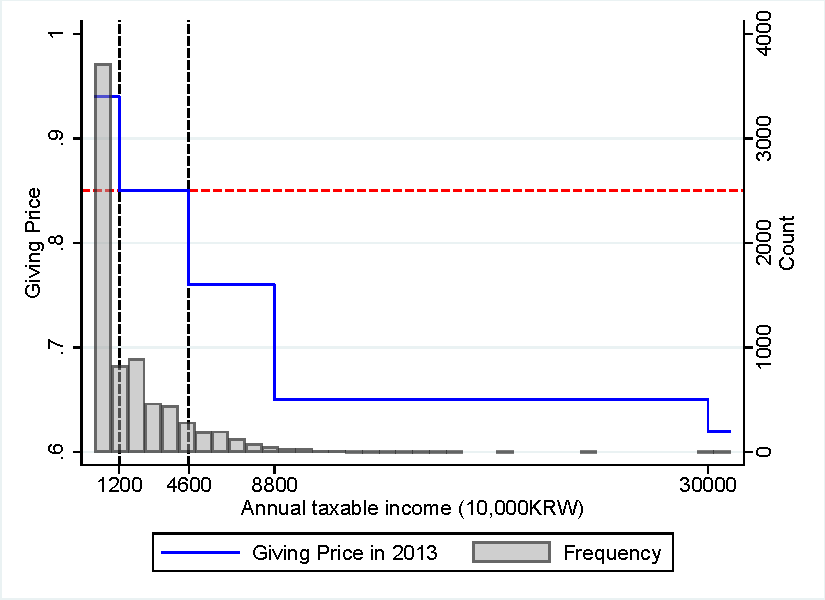
\includegraphics[width=0.9\linewidth]{C:/Users/vge00/Desktop/NaSTaB/_assets/SummaryPriceChange} 
  
  }
  
  \caption{Income Distribution and Giving Price in 2013}\label{fig:unnamed-chunk-2}
  \end{figure}
  
  \hypertarget{main-results}{%
  \section{Main Results}\label{main-results}}
  
  \begin{figure}
  
  {\centering 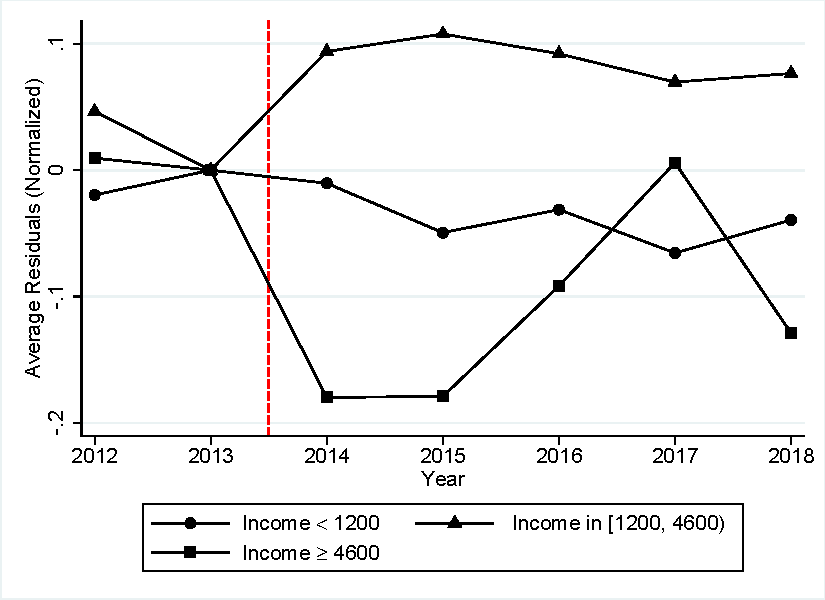
\includegraphics[width=0.9\linewidth]{C:/Users/vge00/Desktop/NaSTaB/_assets/ElasticityResid} 
  
  }
  
  \caption{Average Residuals Grouped by Year and Tax-Reform Benefit Group}\label{fig:unnamed-chunk-3}
  \end{figure}
  
  \begin{table}
  
  \caption{\label{tab:kableEstimateElasticityPart1}Main Results}
  \centering
  \fontsize{8}{10}\selectfont
  \begin{threeparttable}
  \begin{tabular}[t]{lccccc}
  \toprule
   & (1) & (2) & (3) & (4) & (5)\\
  \midrule
  ln(giving price) & -1.072*** & -1.264*** & -1.291*** & -1.114*** & -1.241***\\
   & (0.202) & (0.213) & (0.230) & (0.229) & (0.227)\\
  ln(auunaul taxable income) & 5.392*** & 5.080*** & 5.047*** & 5.116*** & 4.946***\\
   & (0.970) & (0.964) & (0.964) & (0.966) & (0.949)\\
  Individual FE & Y & Y & Y & Y & Y\\
  Time FE & Y & Y & Y & Y & Y\\
  Age & N & Y & Y & Y & Y\\
  Year X Education & N & N & Y & Y & Y\\
  Year X Gender & N & N & N & Y & Y\\
  Year X Resident Area & N & N & N & N & Y\\
  N & 53269 & 53269 & 53267 & 53267 & 53267\\
  R-sq & 0.009 & 0.010 & 0.010 & 0.011 & 0.020\\
  \bottomrule
  \end{tabular}
  \begin{tablenotes}
  \item Notes: $^{*}$ $p < 0.1$, $^{**}$ $p < 0.05$, $^{***}$ $p < 0.01$. Standard errors are clustered at individual level. When controlling age, we alson include its squared term.
  \end{tablenotes}
  \end{threeparttable}
  \end{table}
  
  \begin{figure}
  
  {\centering 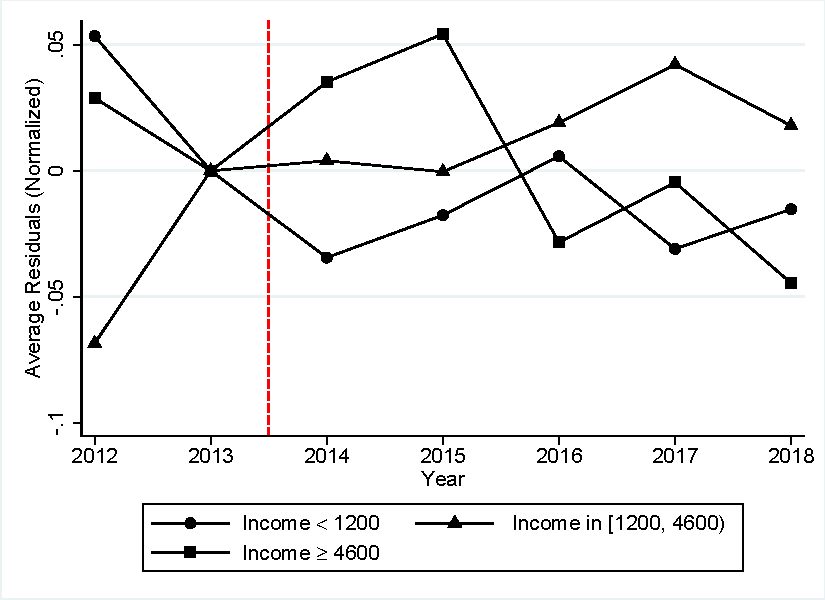
\includegraphics[width=0.9\linewidth]{C:/Users/vge00/Desktop/NaSTaB/_assets/IntElasticityResid} 
  
  }
  
  \caption{Average Residuals Grouped by Year and Tax-Reform Benefit Group (Intensive Margin)}\label{fig:unnamed-chunk-4}
  \end{figure}
  
  \begin{figure}
  
  {\centering 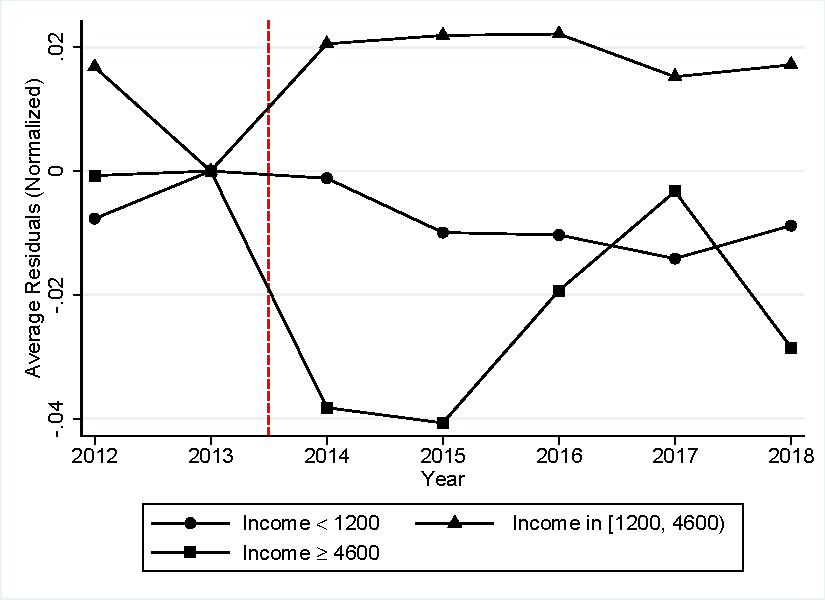
\includegraphics[width=0.9\linewidth]{C:/Users/vge00/Desktop/NaSTaB/_assets/ExtElasticityResid} 
  
  }
  
  \caption{Average Residuals Grouped by Year and Tax-Reform Benefit Group (Extensive Margin)}\label{fig:unnamed-chunk-5}
  \end{figure}
  
  \begin{table}
  
  \caption{\label{tab:kableEstimateElasticityPart2}Main Results: Intensive- and Extensive-Margin Elasticity}
  \centering
  \fontsize{8}{10}\selectfont
  \begin{threeparttable}
  \begin{tabular}[t]{lccccc}
  \toprule
   & (1) & (2) & (3) & (4) & (5)\\
  \midrule
  \addlinespace[0.3em]
  \multicolumn{6}{l}{\textbf{Intensive-Margin Elasticity}}\\
  \hspace{1em}ln(giving price) & -0.593*** & -0.838*** & -1.016*** & -0.893*** & -0.904***\\
  \hspace{1em} & (0.203) & (0.212) & (0.232) & (0.243) & (0.248)\\
  \hspace{1em}ln(auunaul taxable income) & 2.015*** & 1.562** & 1.445** & 1.528** & 1.571**\\
  \hspace{1em} & (0.675) & (0.655) & (0.647) & (0.651) & (0.653)\\
  \hspace{1em}N & 11637 & 11637 & 11637 & 11637 & 11637\\
  \hspace{1em}R-sq & 0.006 & 0.009 & 0.012 & 0.013 & 0.034\\
  \addlinespace[0.3em]
  \multicolumn{6}{l}{\textbf{Extensive-Margin Elasticity}}\\
  \hspace{1em}ln(giving price) & -0.257*** & -0.288*** & -0.273*** & -0.237*** & -0.267***\\
  \hspace{1em} & (0.046) & (0.048) & (0.052) & (0.052) & (0.051)\\
  \hspace{1em}ln(auunaul taxable income) & 1.175*** & 1.124*** & 1.125*** & 1.139*** & 1.102***\\
  \hspace{1em} & (0.223) & (0.223) & (0.223) & (0.224) & (0.220)\\
  \hspace{1em}Implied price elasiticity & -1.264*** & -1.418*** & -1.343*** & -1.167*** & -1.312***\\
  \hspace{1em} & (0.226) & (0.237) & (0.256) & (0.256) & (0.253)\\
  \hspace{1em}Implied income elasticity & 5.778*** & 5.527*** & 5.531*** & 5.600*** & 5.420***\\
  \hspace{1em} & (1.099) & (1.097) & (1.099) & (1.100) & (1.080)\\
  \hspace{1em}Individual FE & Y & Y & Y & Y & Y\\
  \hspace{1em}Time FE & Y & Y & Y & Y & Y\\
  \hspace{1em}Age & N & Y & Y & Y & Y\\
  \hspace{1em}Year X Education & N & N & Y & Y & Y\\
  \hspace{1em}Year X Gender & N & N & N & Y & Y\\
  \hspace{1em}Year X Resident Area & N & N & N & N & Y\\
  \hspace{1em}N & 53269 & 53269 & 53267 & 53267 & 53267\\
  \hspace{1em}R-sq & 0.008 & 0.009 & 0.009 & 0.010 & 0.019\\
  \bottomrule
  \end{tabular}
  \begin{tablenotes}
  \item Notes: $^{*}$ $p < 0.1$, $^{**}$ $p < 0.05$, $^{***}$ $p < 0.01$. Standard errors are clustered at individual level. When controlling age, we alson include its squared term. The implied extensive-marign price elasticity is evaluated at the sample mean of $D_{ijt}$.
  \end{tablenotes}
  \end{threeparttable}
  \end{table}
  
  \begin{table}
  
  \caption{\label{tab:kableLastElasticity1}Last Price Elasticity: Panel IV}
  \centering
  \fontsize{8}{10}\selectfont
  \begin{threeparttable}
  \begin{tabular}[t]{lccccc}
  \toprule
   & (1) & (2) & (3) & (4) & (5)\\
  \midrule
  ln(last giving price) & -2.421*** & -2.536*** & -2.750*** & -2.529*** & -2.650***\\
   & (0.204) & (0.216) & (0.233) & (0.231) & (0.229)\\
  ln(auunaul taxable income) & 5.258*** & 5.071*** & 4.981*** & 5.058*** & 4.910***\\
   & (0.961) & (0.961) & (0.959) & (0.961) & (0.948)\\
  Individual FE & Y & Y & Y & Y & Y\\
  Time FE & Y & Y & Y & Y & Y\\
  Age & N & Y & Y & Y & Y\\
  Year X Education & N & N & Y & Y & Y\\
  Year X Gender & N & N & N & Y & Y\\
  Year X Resident Area & N & N & N & N & Y\\
  F-statistics of IV & 149708.36 & 133463.98 & 122042.55 & 119684.05 & 115742.55\\
  N & 52304 & 52304 & 52302 & 52302 & 52302\\
  \bottomrule
  \end{tabular}
  \begin{tablenotes}
  \item Notes: $^{*}$ $p < 0.1$, $^{**}$ $p < 0.05$, $^{***}$ $p < 0.01$. Standard errors are clustered at individual level. The instumental variable is the first giving price in year $t$. When controlling age, we alson include its squared term.
  \end{tablenotes}
  \end{threeparttable}
  \end{table}
  
  \begin{table}
  
  \caption{\label{tab:kableLastElasticity2}Intensive- and Extensive-Margin Last Price Elasticity: Panel IV}
  \centering
  \fontsize{8}{10}\selectfont
  \begin{threeparttable}
  \begin{tabular}[t]{lccccc}
  \toprule
   & (1) & (2) & (3) & (4) & (5)\\
  \midrule
  \addlinespace[0.3em]
  \multicolumn{6}{l}{\textbf{Intensive-Margin Elasticity}}\\
  \hspace{1em}ln(last giving price) & -0.898*** & -0.961*** & -1.197*** & -0.998*** & -1.074***\\
  \hspace{1em} & (0.271) & (0.271) & (0.307) & (0.325) & (0.332)\\
  \hspace{1em}ln(auunaul taxable income) & 2.023*** & 1.638** & 1.460** & 1.530** & 1.572**\\
  \hspace{1em} & (0.694) & (0.678) & (0.667) & (0.670) & (0.667)\\
  \hspace{1em}F-statistics of IV & 8861.30 & 8893.12 & 7522.05 & 6585.00 & 6426.96\\
  \hspace{1em}N & 10672 & 10672 & 10672 & 10672 & 10672\\
  \addlinespace[0.3em]
  \multicolumn{6}{l}{\textbf{Extensive-Margin Elasticity}}\\
  \hspace{1em}ln(last giving price) & -0.623*** & -0.630*** & -0.644*** & -0.593*** & -0.619***\\
  \hspace{1em} & (0.046) & (0.049) & (0.053) & (0.052) & (0.052)\\
  \hspace{1em}ln(auunaul taxable income) & 1.125*** & 1.113*** & 1.103*** & 1.121*** & 1.090***\\
  \hspace{1em} & (0.221) & (0.223) & (0.223) & (0.223) & (0.220)\\
  \hspace{1em}Implied last price elasiticity & -3.063*** & -3.100*** & -3.167*** & -2.917*** & -3.046***\\
  \hspace{1em} & (0.227) & (0.240) & (0.259) & (0.258) & (0.254)\\
  \hspace{1em}Implied income elasticity & 5.532*** & 5.472*** & 5.426*** & 5.513*** & 5.361***\\
  \hspace{1em} & (1.088) & (1.096) & (1.096) & (1.098) & (1.082)\\
  \hspace{1em}Individual FE & Y & Y & Y & Y & Y\\
  \hspace{1em}Time FE & Y & Y & Y & Y & Y\\
  \hspace{1em}Age & N & Y & Y & Y & Y\\
  \hspace{1em}Year X Education & N & N & Y & Y & Y\\
  \hspace{1em}Year X Gender & N & N & N & Y & Y\\
  \hspace{1em}Year X Resident Area & N & N & N & N & Y\\
  \hspace{1em}F-statistics of IV & 149708.36 & 133463.98 & 122042.55 & 119684.05 & 115742.55\\
  \hspace{1em}N & 52304 & 52304 & 52302 & 52302 & 52302\\
  \bottomrule
  \end{tabular}
  \begin{tablenotes}
  \item Notes: $^{*}$ $p < 0.1$, $^{**}$ $p < 0.05$, $^{***}$ $p < 0.01$. Standard errors are clustered at individual level. The instumental variable is the first giving price in year $t$. When controlling age, we alson include its squared term. The implied extensive-marign price elasticity is evaluated at the sample mean of $D_{ijt}$.
  \end{tablenotes}
  \end{threeparttable}
  \end{table}
  
  \begin{table}
  
  \caption{\label{tab:kableShortElasticity1}Elasticity with Short-Period Data}
  \centering
  \fontsize{8}{10}\selectfont
  \begin{threeparttable}
  \begin{tabular}[t]{lcccc}
  \toprule
  \multicolumn{1}{c}{ } & \multicolumn{2}{c}{After 2012} & \multicolumn{2}{c}{2013 and 2014} \\
  \cmidrule(l{3pt}r{3pt}){2-3} \cmidrule(l{3pt}r{3pt}){4-5}
   & (1) & (2) & (3) & (4)\\
  \midrule
  ln(giving price) & -1.014*** & -1.286*** & -1.398*** & -1.686***\\
   & (0.255) & (0.290) & (0.289) & (0.338)\\
  ln(auunaul taxable income) & 5.108*** & 4.743*** & 4.013** & 3.035\\
   & (1.009) & (0.990) & (1.948) & (1.992)\\
  Individual FE & Y & Y & Y & Y\\
  Time FE & Y & Y & Y & Y\\
  Other Controls & N & Y & N & Y\\
  N & 45994 & 45992 & 14893 & 14893\\
  R-sq & 0.009 & 0.018 & 0.013 & 0.024\\
  \bottomrule
  \end{tabular}
  \begin{tablenotes}
  \item Notes: $^{*}$ $p < 0.1$, $^{**}$ $p < 0.05$, $^{***}$ $p < 0.01$. Standard errors are clustered at individual level. Other controls are age (its squared value), the interaction between year dummies and education dummies, the interaction between year dummies and gender dummies, and the interaction between year dummies and resident area.
  \end{tablenotes}
  \end{threeparttable}
  \end{table}
  
  \begin{table}
  
  \caption{\label{tab:kableShortElasticity2}Intensive- and Extensive-Margin Elasticity with Short-Period Data}
  \centering
  \fontsize{8}{10}\selectfont
  \begin{threeparttable}
  \begin{tabular}[t]{lcccc}
  \toprule
  \multicolumn{1}{c}{ } & \multicolumn{2}{c}{After 2012} & \multicolumn{2}{c}{2013 and 2014} \\
  \cmidrule(l{3pt}r{3pt}){2-3} \cmidrule(l{3pt}r{3pt}){4-5}
   & (1) & (2) & (3) & (4)\\
  \midrule
  \addlinespace[0.3em]
  \multicolumn{5}{l}{\textbf{Intensive-Margin Elasticity}}\\
  \hspace{1em}ln(giving price) & -0.647*** & -1.129*** & -0.394 & -0.712**\\
  \hspace{1em} & (0.236) & (0.291) & (0.310) & (0.363)\\
  \hspace{1em}ln(auunaul taxable income) & 1.943*** & 1.714*** & 1.440 & 1.047\\
  \hspace{1em} & (0.662) & (0.649) & (2.975) & (3.072)\\
  \hspace{1em}N & 10158 & 10158 & 2922 & 2922\\
  \hspace{1em}R-sq & 0.006 & 0.034 & 0.004 & 0.046\\
  \addlinespace[0.3em]
  \multicolumn{5}{l}{\textbf{Extensive-Margin Elasticity}}\\
  \hspace{1em}ln(giving price) & -0.235*** & -0.269*** & -0.331*** & -0.383***\\
  \hspace{1em} & (0.058) & (0.065) & (0.065) & (0.076)\\
  \hspace{1em}ln(auunaul taxable income) & 1.093*** & 1.024*** & 0.801* & 0.574\\
  \hspace{1em} & (0.230) & (0.226) & (0.428) & (0.447)\\
  \hspace{1em}Implied price elasiticity & -1.136*** & -1.300*** & -1.845*** & -2.131***\\
  \hspace{1em} & (0.279) & (0.314) & (0.364) & (0.422)\\
  \hspace{1em}Implied income elasticity & 5.287*** & 4.954*** & 4.457* & 3.196\\
  \hspace{1em} & (1.114) & (1.094) & (2.381) & (2.488)\\
  \hspace{1em}Individual FE & Y & Y & Y & Y\\
  \hspace{1em}Time FE & Y & Y & Y & Y\\
  \hspace{1em}Other Controls & N & Y & N & Y\\
  \hspace{1em}N & 45994 & 45992 & 14893 & 14893\\
  \hspace{1em}R-sq & 0.008 & 0.018 & 0.013 & 0.022\\
  \bottomrule
  \end{tabular}
  \begin{tablenotes}
  \item Notes: $^{*}$ $p < 0.1$, $^{**}$ $p < 0.05$, $^{***}$ $p < 0.01$. Standard errors are clustered at individual level. Other controls are age (its squared value), the interaction between year dummies and education dummies, the interaction between year dummies and gender dummies, and the interaction between year dummies and resident area. The implied extensive-marign price elasticity is evaluated at the sample mean of $D_{ijt}$.
  \end{tablenotes}
  \end{threeparttable}
  \end{table}
  
  \begin{table}
  
  \caption{\label{tab:kablekDiffElasticity}Estimation of Elasticity: $k$-difference model}
  \centering
  \fontsize{8}{10}\selectfont
  \begin{threeparttable}
  \begin{tabular}[t]{lccc}
  \toprule
  \multicolumn{1}{c}{lag $k$} & \multicolumn{1}{c}{$k = 1$} & \multicolumn{1}{c}{$k = 2$} & \multicolumn{1}{c}{$k = 3$} \\
  \cmidrule(l{3pt}r{3pt}){1-1} \cmidrule(l{3pt}r{3pt}){2-2} \cmidrule(l{3pt}r{3pt}){3-3} \cmidrule(l{3pt}r{3pt}){4-4}
   & (1) & (2) & (3)\\
  \midrule
  \addlinespace[0.3em]
  \multicolumn{4}{l}{\textbf{Overall Elasticity}}\\
  \hspace{1em}Lagged difference of first price (log) & -1.894*** & -2.170*** & -1.752***\\
  \hspace{1em} & (0.389) & (0.355) & (0.346)\\
  \hspace{1em}Lagged difference of annual income (log) & 2.737*** & 4.685*** & 5.307***\\
  \hspace{1em} & (1.042) & (1.141) & (1.174)\\
  \hspace{1em}N & 49014 & 46610 & 44205\\
  \hspace{1em}R-sq & 0.010 & 0.015 & 0.015\\
  \addlinespace[0.3em]
  \multicolumn{4}{l}{\textbf{Intensive-Margin Elasticity}}\\
  \hspace{1em}Lagged difference of first price (log) & -1.854** & -2.282*** & -2.163***\\
  \hspace{1em} & (0.763) & (0.621) & (0.550)\\
  \hspace{1em}Lagged difference of annual income (log) & 2.229 & 4.675*** & 5.582**\\
  \hspace{1em} & (1.715) & (1.791) & (2.178)\\
  \hspace{1em}Individual FE & Y & Y & Y\\
  \hspace{1em}Time FE & Y & Y & Y\\
  \hspace{1em}Other Controls & Y & Y & Y\\
  \hspace{1em}N & 10939 & 10505 & 10043\\
  \hspace{1em}R-sq & 0.066 & 0.073 & 0.055\\
  \bottomrule
  \end{tabular}
  \begin{tablenotes}
  \item Notes: $^{*}$ $p < 0.1$, $^{**}$ $p < 0.05$, $^{***}$ $p < 0.01$. Standard errors are clustered at individual level. The lagged difference of first price (log) is $\ln(\text{Price}^k_{ijt}) - \ln(\text{Price}_{ij(t-k)})$, where $\text{Price}^k_{ijt}$ calculates the giving price under the tax system in year $t$, using annual taxable income in year $t-k$, $\text{Income}_{ij(t-k)}$. The lagged of annual income (log) is $\ln(\text{Income}_{ijt}) - \ln(\text{Income}_{ij(t-k)})$. Other controls are lagged difference of age, lagged difference of squared age, the interaction between year dummies and education dummies, the interaction between year dummies and gender dummies, and the interaction between year dummies and resident area.
  \end{tablenotes}
  \end{threeparttable}
  \end{table}
  
  \hypertarget{governement-efficient-and-price-elasticity}{%
  \section{Governement Efficient and Price Elasticity}\label{governement-efficient-and-price-elasticity}}
  
  \begin{figure}
  
  {\centering 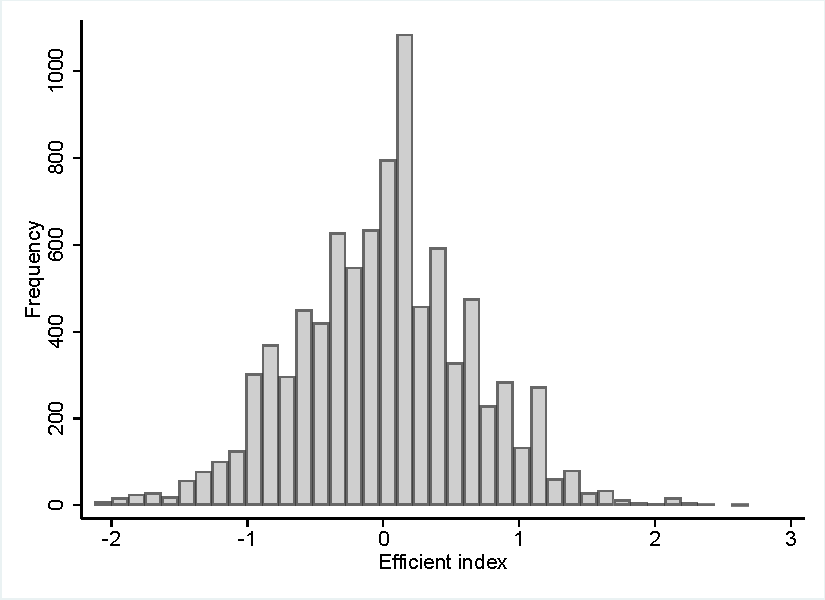
\includegraphics[width=0.9\linewidth]{C:/Users/vge00/Desktop/NaSTaB/_assets/HistogramEfficientid} 
  
  }
  
  \caption{Histogram of Efficient Index}\label{fig:unnamed-chunk-6}
  \end{figure}
  
  \begin{table}
  
  \caption{\label{tab:kableHeteroElasticity}Heterogenous Elasticity by Perceived Government Efficiency}
  \centering
  \fontsize{8}{10}\selectfont
  \begin{threeparttable}
  \begin{tabular}[t]{lccc}
  \toprule
  \multicolumn{1}{c}{ } & \multicolumn{1}{c}{Overall} & \multicolumn{1}{c}{Extensive} & \multicolumn{1}{c}{Intensive} \\
  \cmidrule(l{3pt}r{3pt}){2-2} \cmidrule(l{3pt}r{3pt}){3-3} \cmidrule(l{3pt}r{3pt}){4-4}
   & (1) & (2) & (3)\\
  \midrule
  ln(giving price) & -1.356*** & -0.284*** & -0.952***\\
   & (0.336) & (0.076) & (0.334)\\
  ln(giving price) X 2Q Efficient Group & -0.032 & -0.059 & 0.292\\
   & (0.423) & (0.098) & (0.489)\\
  ln(giving price) X 3Q Efficient Group & 0.353 & 0.095 & -0.285\\
   & (0.417) & (0.097) & (0.545)\\
  ln(auunaul taxable income) & 4.943*** & 1.104*** & 1.589**\\
   & (0.959) & (0.222) & (0.657)\\
  Implied price elasiticity (1Q efficient group) & -1.356*** & -1.396*** & -0.952***\\
   & (0.336) & (0.374) & (0.334)\\
  Implied price elasiticity (2Q efficient group) & -1.388*** & -1.686*** & -0.661*\\
   & (0.330) & (0.378) & (0.394)\\
  Implied price elasiticity (3Q efficient group) & -1.002*** & -0.930** & -1.237***\\
   & (0.327) & (0.374) & (0.468)\\
  Implied income elasticity & 4.943*** & 5.429*** & 1.589**\\
   & (0.959) & (1.093) & (0.657)\\
  Individual FE & Y & Y & Y\\
  Time FE & Y & Y & Y\\
  Other Controls & Y & Y & Y\\
  N & 50455 & 50455 & 11327\\
  R-sq & 0.020 & 0.020 & 0.034\\
  \bottomrule
  \end{tabular}
  \begin{tablenotes}
  \item Notes: $^{*}$ $p < 0.1$, $^{**}$ $p < 0.05$, $^{***}$ $p < 0.01$. Standard errors are clustered at individual level. The 2Q (3Q) Efficient Group is a dummy varaible taking 1 if individual $i$ belongs to the second (third) quanitle of efficient index. Other controls are age (its squared value), the interaction between year dummies and education dummies, the interaction between year dummies and gender dummies, and the interaction between year dummies and resident area. The implied extensive-margin elasticity is evaluated at the sample mean of $D_{ijt}$.
  \end{tablenotes}
  \end{threeparttable}
  \end{table}
  
  \begin{figure}
  
  {\centering 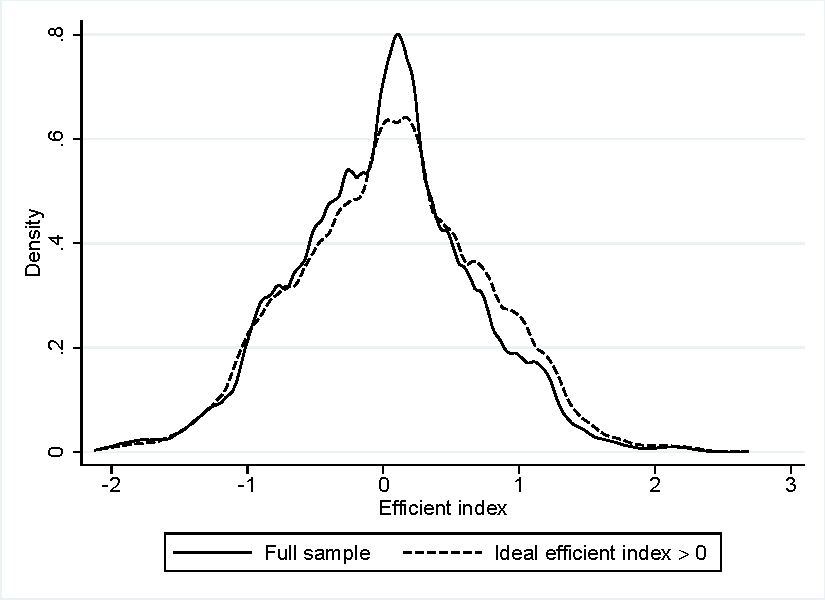
\includegraphics[width=0.9\linewidth]{C:/Users/vge00/Desktop/NaSTaB/_assets/DensityEfficientid} 
  
  }
  
  \caption{Density of Efficient Index Using those whose ideal efficient index > 0}\label{fig:unnamed-chunk-7}
  \end{figure}
  
  \begin{table}
  
  \caption{\label{tab:kableSubsetHeteroElasticity}Heterogenous Elasticity Using Those whose Ideal Efficient Index > 0}
  \centering
  \fontsize{8}{10}\selectfont
  \begin{threeparttable}
  \begin{tabular}[t]{lccc}
  \toprule
  \multicolumn{1}{c}{ } & \multicolumn{1}{c}{Overall} & \multicolumn{1}{c}{Extensive} & \multicolumn{1}{c}{Intensive} \\
  \cmidrule(l{3pt}r{3pt}){2-2} \cmidrule(l{3pt}r{3pt}){3-3} \cmidrule(l{3pt}r{3pt}){4-4}
   & (1) & (2) & (3)\\
  \midrule
  ln(giving price) & -1.831*** & -0.316*** & -1.303**\\
   & (0.538) & (0.115) & (0.571)\\
  ln(giving price) X 2Q Efficient Group & 0.339 & 0.045 & 0.308\\
   & (0.657) & (0.146) & (0.807)\\
  ln(giving price) X 3Q Efficient Group & 1.295** & 0.237* & 0.236\\
   & (0.586) & (0.135) & (0.834)\\
  ln(auunaul taxable income) & 5.686*** & 1.202*** & 3.225*\\
   & (1.272) & (0.273) & (1.880)\\
  Implied price elasiticity (1Q efficient group) & -1.831*** & -1.555*** & -1.303**\\
   & (0.538) & (0.565) & (0.571)\\
  Implied price elasiticity (2Q efficient group) & -1.492*** & -1.335** & -0.995\\
   & (0.505) & (0.561) & (0.622)\\
  Implied price elasiticity (3Q efficient group) & -0.536 & -0.392 & -1.067\\
   & (0.416) & (0.500) & (0.680)\\
  Implied income elasticity & 5.686*** & 5.913*** & 3.225*\\
   & (1.272) & (1.344) & (1.880)\\
  Individual FE & Y & Y & Y\\
  Time FE & Y & Y & Y\\
  Other Controls & Y & Y & Y\\
  N & 23366 & 23366 & 5004\\
  R-sq & 0.020 & 0.019 & 0.057\\
  \bottomrule
  \end{tabular}
  \begin{tablenotes}
  \item Notes: $^{*}$ $p < 0.1$, $^{**}$ $p < 0.05$, $^{***}$ $p < 0.01$. Standard errors are clustered at individual level. The 2Q (3Q) Efficient Group is a dummy varaible taking 1 if individual $i$ belongs to the second (third) quanitle of efficient index. Other controls are age (its squared value), the interaction between year dummies and education dummies, the interaction between year dummies and gender dummies, and the interaction between year dummies and resident area. We drop units whose the ideal efficient index is less than or equal to zero. The implied extensive-margin elasticity is evaluated at the sample mean of $D_{ijt}$.
  \end{tablenotes}
  \end{threeparttable}
  \end{table}
  
  \begin{table}
  
  \caption{\label{tab:kableHeteroLastElasticity}Heterogenous Last Price Elasticity: Panel IV}
  \centering
  \fontsize{8}{10}\selectfont
  \begin{threeparttable}
  \begin{tabular}[t]{lcccccc}
  \toprule
  \multicolumn{1}{c}{ } & \multicolumn{3}{c}{Full Sample} & \multicolumn{3}{c}{Ideal Efficient Index > 0} \\
  \cmidrule(l{3pt}r{3pt}){2-4} \cmidrule(l{3pt}r{3pt}){5-7}
  \multicolumn{1}{c}{ } & \multicolumn{1}{c}{Overall} & \multicolumn{1}{c}{Extensive} & \multicolumn{1}{c}{Intensive} & \multicolumn{1}{c}{Overall} & \multicolumn{1}{c}{Extensive} & \multicolumn{1}{c}{Intensive} \\
  \cmidrule(l{3pt}r{3pt}){2-2} \cmidrule(l{3pt}r{3pt}){3-3} \cmidrule(l{3pt}r{3pt}){4-4} \cmidrule(l{3pt}r{3pt}){5-5} \cmidrule(l{3pt}r{3pt}){6-6} \cmidrule(l{3pt}r{3pt}){7-7}
   & (1) & (2) & (3) & (4) & (5) & (6)\\
  \midrule
  ln(last giving price) & -2.604*** & -0.586*** & -1.166*** & -2.984*** & -0.579*** & -1.681**\\
   & (0.342) & (0.077) & (0.438) & (0.551) & (0.116) & (0.778)\\
  ln(last giving price) X 2Q Efficient Group & -0.272 & -0.104 & 0.043 & -0.108 & -0.063 & 0.239\\
   & (0.417) & (0.095) & (0.591) & (0.645) & (0.141) & (1.019)\\
  ln(last giving price) X 3Q Efficient Group & -0.010 & -0.038 & 0.111 & 0.894 & 0.056 & 1.285\\
   & (0.420) & (0.096) & (0.709) & (0.588) & (0.132) & (1.071)\\
  ln(auunaul taxable income) & 4.892*** & 1.087*** & 1.597** & 5.313*** & 1.141*** & 2.743\\
   & (0.958) & (0.222) & (0.670) & (1.282) & (0.277) & (1.947)\\
  Implied last price elasiticity (1Q efficient group) & -2.604*** & -2.883*** & -1.166*** & -2.984*** & -3.097*** & -1.681**\\
   & (0.342) & (0.377) & (0.438) & (0.551) & (0.621) & (0.778)\\
  Implied last price elasiticity (2Q efficient group) & -2.876*** & -3.395*** & -1.122** & -3.092*** & -3.432*** & -1.442*\\
   & (0.318) & (0.362) & (0.488) & (0.491) & (0.583) & (0.776)\\
  Implied last price elasiticity (3Q efficient group) & -2.614*** & -3.071*** & -1.055* & -2.091*** & -2.796*** & -0.396\\
   & (0.328) & (0.371) & (0.639) & (0.414) & (0.533) & (0.892)\\
  Implied income elasticity & 4.892*** & 5.345*** & 1.597** & 5.313*** & 6.097*** & 2.743\\
   & (0.958) & (1.094) & (0.670) & (1.282) & (1.481) & (1.947)\\
  Individual FE & Y & Y & Y & Y & Y & Y\\
  Time FE & Y & Y & Y & Y & Y & Y\\
  Other Controls & Y & Y & Y & Y & Y & Y\\
  N & 49575 & 49575 & 10447 & 22974 & 22974 & 4612\\
  \bottomrule
  \end{tabular}
  \begin{tablenotes}
  \item Notes: $^{*}$ $p < 0.1$, $^{**}$ $p < 0.05$, $^{***}$ $p < 0.01$. Standard errors are clustered at individual level. The 2Q (3Q) Efficient Group is a dummy varaible taking 1 if individual $i$ belongs to the second (third) quanitle of efficient index. Other controls are age (its squared value), the interaction between year dummies and education dummies, the interaction between year dummies and gender dummies, and the interaction between year dummies and resident area. The instumental variables are the first giving price in year $t$ and its interaction with the 2Q (3Q) Efficient Group. We drop units whose the ideal efficient index is less than or equal to zero in column (4)-(6). The implied extensive-margin elasticity is evaluated at the sample mean of $D_{ijt}$.
  \end{tablenotes}
  \end{threeparttable}
  \end{table}
  
  \begin{table}
  
  \caption{\label{tab:kableHeteroShortElasticity}Heterogenous Price Elasticity with Data after 2012}
  \centering
  \fontsize{8}{10}\selectfont
  \begin{threeparttable}
  \begin{tabular}[t]{lcccccc}
  \toprule
  \multicolumn{1}{c}{ } & \multicolumn{3}{c}{Full Sample} & \multicolumn{3}{c}{Ideal Efficient Index > 0} \\
  \cmidrule(l{3pt}r{3pt}){2-4} \cmidrule(l{3pt}r{3pt}){5-7}
  \multicolumn{1}{c}{ } & \multicolumn{1}{c}{Overall} & \multicolumn{1}{c}{Extensive} & \multicolumn{1}{c}{Intensive} & \multicolumn{1}{c}{Overall} & \multicolumn{1}{c}{Extensive} & \multicolumn{1}{c}{Intensive} \\
  \cmidrule(l{3pt}r{3pt}){2-2} \cmidrule(l{3pt}r{3pt}){3-3} \cmidrule(l{3pt}r{3pt}){4-4} \cmidrule(l{3pt}r{3pt}){5-5} \cmidrule(l{3pt}r{3pt}){6-6} \cmidrule(l{3pt}r{3pt}){7-7}
   & (1) & (2) & (3) & (4) & (5) & (6)\\
  \midrule
  ln(giving price) & -1.116*** & -0.197** & -1.175*** & -1.526** & -0.187 & -1.301*\\
   & (0.425) & (0.096) & (0.380) & (0.650) & (0.146) & (0.713)\\
  ln(giving price) X 2Q Efficient Group & -0.499 & -0.198 & 0.164 & 0.064 & -0.090 & -0.094\\
   & (0.544) & (0.124) & (0.558) & (0.863) & (0.192) & (0.974)\\
  ln(giving price) X 3Q Efficient Group & -0.125 & -0.060 & -0.167 & 0.448 & -0.036 & 0.197\\
   & (0.530) & (0.124) & (0.630) & (0.733) & (0.175) & (0.941)\\
  ln(auunaul taxable income) & 4.777*** & 1.034*** & 1.757*** & 6.126*** & 1.239*** & 2.903\\
   & (1.002) & (0.229) & (0.652) & (1.414) & (0.305) & (2.188)\\
  Implied price elasiticity (1Q efficient group) & -1.116*** & -0.951** & -1.175*** & -1.526** & -1.000 & -1.301*\\
   & (0.425) & (0.464) & (0.380) & (0.650) & (0.780) & (0.713)\\
  Implied price elasiticity (2Q efficient group) & -1.615*** & -1.910*** & -1.011** & -1.462** & -1.480* & -1.394*\\
   & (0.431) & (0.470) & (0.455) & (0.730) & (0.835) & (0.755)\\
  Implied price elasiticity (3Q efficient group) & -1.240*** & -1.242*** & -1.342** & -1.078* & -1.193* & -1.103\\
   & (0.413) & (0.470) & (0.549) & (0.550) & (0.722) & (0.739)\\
  Implied income elasticity & 4.777*** & 4.998*** & 1.757*** & 6.126*** & 6.622*** & 2.903\\
   & (1.002) & (1.107) & (0.652) & (1.414) & (1.632) & (2.188)\\
  Individual FE & Y & Y & Y & Y & Y & Y\\
  Time FE & Y & Y & Y & Y & Y & Y\\
  Other Controls & Y & Y & Y & Y & Y & Y\\
  N & 44115 & 44115 & 9967 & 20441 & 20441 & 4419\\
  R-sq & 0.018 & 0.019 & 0.034 & 0.018 & 0.018 & 0.061\\
  \bottomrule
  \end{tabular}
  \begin{tablenotes}
  \item Notes: $^{*}$ $p < 0.1$, $^{**}$ $p < 0.05$, $^{***}$ $p < 0.01$. Standard errors are clustered at individual level. The 2Q (3Q) Efficient Group is a dummy varaible taking 1 if individual $i$ belongs to the second (third) quanitle of efficient index. Other controls are age (its squared value), the interaction between year dummies and education dummies, the interaction between year dummies and gender dummies, and the interaction between year dummies and resident area. We drop units whose the ideal efficient index is less than or equal to zero in column (4)-(6). The implied extensive-margin elasticity is evaluated at the sample mean of $D_{ijt}$.
  \end{tablenotes}
  \end{threeparttable}
  \end{table}
  
  \begin{table}
  
  \caption{\label{tab:kableHeterokDiffElasticity}Heterogenous Price Elasticity: $k$-difference Model}
  \centering
  \fontsize{8}{10}\selectfont
  \begin{threeparttable}
  \begin{tabular}[t]{lcccccc}
  \toprule
  \multicolumn{1}{c}{ } & \multicolumn{3}{c}{Overall Elasticity} & \multicolumn{3}{c}{Intensive-Margin Elasticity} \\
  \cmidrule(l{3pt}r{3pt}){2-4} \cmidrule(l{3pt}r{3pt}){5-7}
  \multicolumn{1}{c}{Lag $k$} & \multicolumn{1}{c}{$k = 1$} & \multicolumn{1}{c}{$k = 2$} & \multicolumn{1}{c}{$k = 3$} & \multicolumn{1}{c}{$k = 1$} & \multicolumn{1}{c}{$k = 2$} & \multicolumn{1}{c}{$k = 3$} \\
  \cmidrule(l{3pt}r{3pt}){1-1} \cmidrule(l{3pt}r{3pt}){2-2} \cmidrule(l{3pt}r{3pt}){3-3} \cmidrule(l{3pt}r{3pt}){4-4} \cmidrule(l{3pt}r{3pt}){5-5} \cmidrule(l{3pt}r{3pt}){6-6} \cmidrule(l{3pt}r{3pt}){7-7}
   & (1) & (2) & (3) & (4) & (5) & (6)\\
  \midrule
  Lagged difference of first price (log) & -1.778*** & -2.884*** & -2.467*** & -1.401 & -2.320** & -2.549***\\
   & (0.553) & (0.520) & (0.509) & (1.074) & (0.970) & \vphantom{1} (0.788)\\
  \hspace{1em}X 2Q Efficient Group & -0.204 & 0.970 & 0.755 & -0.113 & -0.035 & 0.942\\
   & (0.747) & (0.687) & (0.648) & (1.548) & (1.331) & (1.128)\\
  \hspace{1em}X 3Q Efficient Group & -0.346 & 1.316** & 1.440** & -1.439 & 0.218 & 0.302\\
   & (0.704) & (0.644) & (0.624) & (1.610) & (1.319) & (1.196)\\
  Lagged difference of annual income (log) & 2.685** & 4.641*** & 5.274*** & 2.208 & 4.849*** & 5.471**\\
   & (1.045) & (1.149) & (1.185) & (1.712) & (1.816) & \vphantom{1} (2.189)\\
  Implied price elasiticity (1Q efficient group) & -1.778*** & -2.884*** & -2.467*** & -1.401 & -2.320** & -2.549***\\
   & (0.553) & (0.520) & (0.509) & (1.074) & (0.970) & (0.788)\\
  Implied price elasiticity (2Q efficient group) & -1.982*** & -1.914*** & -1.712*** & -1.515 & -2.355** & -1.607*\\
   & (0.611) & (0.546) & (0.508) & (1.230) & (0.986) & (0.885)\\
  Implied price elasiticity (3Q efficient group) & -2.123*** & -1.568*** & -1.027** & -2.840** & -2.102** & -2.248**\\
   & (0.550) & (0.494) & (0.485) & (1.317) & (0.995) & (0.973)\\
  Implied income elasticity & 2.685** & 4.641*** & 5.274*** & 2.208 & 4.849*** & 5.471**\\
   & (1.045) & (1.149) & (1.185) & (1.712) & (1.816) & (2.189)\\
  Individual FE & Y & Y & Y & Y & Y & Y\\
  Time FE & Y & Y & Y & Y & Y & Y\\
  Other Controls & Y & Y & Y & Y & Y & Y\\
  N & 46661 & 44448 & 42198 & 10675 & 10257 & 9811\\
  R-sq & 0.010 & 0.016 & 0.015 & 0.066 & 0.073 & 0.055\\
  \bottomrule
  \end{tabular}
  \begin{tablenotes}
  \item Notes: $^{*}$ $p < 0.1$, $^{**}$ $p < 0.05$, $^{***}$ $p < 0.01$. Standard errors are clustered at individual level. The 2Q (3Q) Efficient Group is a dummy varaible taking 1 if individual $i$ belongs to the second (third) quanitle of efficient index. The lagged difference of first price (log) is $\ln(\text{Price}^k_{ijt}) - \ln(\text{Price}_{ij(t-k)})$, where $\text{Price}^k_{ijt}$ calculates the giving price under the tax system in year $t$, using annual taxable income in year $t-k$, $\text{Income}_{ij(t-k)}$. The lagged of annual income (log) is $\ln(\text{Income}_{ijt}) - \ln(\text{Income}_{ij(t-k)})$. Other controls are lagged difference of age, lagged difference of squared age, the interaction between year dummies and education dummies, the interaction between year dummies and gender dummies, and the interaction between year dummies and resident area.
  \end{tablenotes}
  \end{threeparttable}
  \end{table}
  
  \begin{table}
  
  \caption{\label{tab:kableSubsetHeterokDiffElasticity}Heterogenous Price Elasticity: $k$-difference Model Using Those whose Ideal Efficient Index > 0}
  \centering
  \fontsize{8}{10}\selectfont
  \begin{threeparttable}
  \begin{tabular}[t]{lcccccc}
  \toprule
  \multicolumn{1}{c}{ } & \multicolumn{3}{c}{Overall Elasticity} & \multicolumn{3}{c}{Intensive-Margin Elasticity} \\
  \cmidrule(l{3pt}r{3pt}){2-4} \cmidrule(l{3pt}r{3pt}){5-7}
  \multicolumn{1}{c}{Lag $k$} & \multicolumn{1}{c}{$k = 1$} & \multicolumn{1}{c}{$k = 2$} & \multicolumn{1}{c}{$k = 3$} & \multicolumn{1}{c}{$k = 1$} & \multicolumn{1}{c}{$k = 2$} & \multicolumn{1}{c}{$k = 3$} \\
  \cmidrule(l{3pt}r{3pt}){1-1} \cmidrule(l{3pt}r{3pt}){2-2} \cmidrule(l{3pt}r{3pt}){3-3} \cmidrule(l{3pt}r{3pt}){4-4} \cmidrule(l{3pt}r{3pt}){5-5} \cmidrule(l{3pt}r{3pt}){6-6} \cmidrule(l{3pt}r{3pt}){7-7}
   & (1) & (2) & (3) & (4) & (5) & (6)\\
  \midrule
  Lagged difference of first price (log) & -2.215** & -3.269*** & -2.647*** & -0.841 & -4.928*** & -2.227\\
   & (0.872) & (0.794) & (0.821) & (1.936) & (1.780) & \vphantom{1} (1.588)\\
  \hspace{1em}X 2Q Efficient Group & 0.078 & 0.900 & 0.604 & -0.752 & 1.312 & -0.954\\
   & (1.233) & (1.070) & (0.972) & (2.841) & (2.329) & (1.992)\\
  \hspace{1em}X 3Q Efficient Group & -0.666 & 2.307*** & 2.242** & -3.101 & 3.154 & 2.071\\
   & (1.024) & (0.894) & (0.875) & (2.646) & (2.219) & (2.081)\\
  Lagged difference of annual income (log) & 3.048** & 5.197*** & 5.749*** & 3.692 & 6.587** & 8.671**\\
   & (1.319) & (1.564) & (1.419) & (4.077) & (3.120) & \vphantom{1} (3.406)\\
  Implied price elasiticity (1Q efficient group) & -2.215** & -3.269*** & -2.647*** & -0.841 & -4.928*** & -2.227\\
   & (0.872) & (0.794) & (0.821) & (1.936) & (1.780) & (1.588)\\
  Implied price elasiticity (2Q efficient group) & -2.137** & -2.369*** & -2.042*** & -1.592 & -3.616** & -3.182**\\
   & (1.064) & (0.869) & (0.725) & (2.238) & (1.656) & (1.336)\\
  Implied price elasiticity (3Q efficient group) & -2.881*** & -0.962 & -0.404 & -3.942* & -1.775 & -0.156\\
   & (0.795) & (0.633) & (0.590) & (2.032) & (1.514) & (1.461)\\
  Implied income elasticity & 3.048** & 5.197*** & 5.749*** & 3.692 & 6.587** & 8.671**\\
   & (1.319) & (1.564) & (1.419) & (4.077) & (3.120) & (3.406)\\
  Individual FE & Y & Y & Y & Y & Y & Y\\
  Time FE & Y & Y & Y & Y & Y & Y\\
  Other Controls & Y & Y & Y & Y & Y & Y\\
  N & 21583 & 20516 & 19422 & 4686 & 4474 & 4245\\
  R-sq & 0.012 & 0.020 & 0.020 & 0.074 & 0.088 & 0.091\\
  \bottomrule
  \end{tabular}
  \begin{tablenotes}
  \item Notes: $^{*}$ $p < 0.1$, $^{**}$ $p < 0.05$, $^{***}$ $p < 0.01$. Standard errors are clustered at individual level. The 2Q (3Q) Efficient Group is a dummy varaible taking 1 if individual $i$ belongs to the second (third) quanitle of efficient index. The lagged difference of first price (log) is $\ln(\text{Price}^k_{ijt}) - \ln(\text{Price}_{ij(t-k)})$, where $\text{Price}^k_{ijt}$ calculates the giving price under the tax system in year $t$, using annual taxable income in year $t-k$, $\text{Income}_{ij(t-k)}$. The lagged of annual income (log) is $\ln(\text{Income}_{ijt}) - \ln(\text{Income}_{ij(t-k)})$. Other controls are lagged difference of age, lagged difference of squared age, the interaction between year dummies and education dummies, the interaction between year dummies and gender dummies, and the interaction between year dummies and resident area. We drop units whose the ideal efficient index is less than or equal to zero.
  \end{tablenotes}
  \end{threeparttable}
  \end{table}
  
  \hypertarget{conclusions}{%
  \section{Conclusions}\label{conclusions}}
  
  \hypertarget{conclusions-1}{%
  \subsection{Conclusions}\label{conclusions-1}}
  
  \clearpage
  
  \hypertarget{references}{%
  \subsection*{References}\label{references}}
  \addcontentsline{toc}{subsection}{References}
  
  \hypertarget{refs}{}
  \leavevmode\hypertarget{ref-Almunia2020}{}%
  Almunia, M., Guceri, I., Lockwood, B., Scharf, K., 2020. More giving or more givers? The effects of tax incentives on charitable donations in the uk. Journal of Public Economics 183. doi:\href{https://doi.org/10.1016/j.jpubeco.2019.104114}{10.1016/j.jpubeco.2019.104114}
  
  \leavevmode\hypertarget{ref-Anderson2017}{}%
  Anderson, J.E., 2017. Trust in government and willingness to pay taxes in transition countries. Comparative Economic Studies 59, 1--22. doi:\href{https://doi.org/10.1057/s41294-016-0017-x}{10.1057/s41294-016-0017-x}
  
  \leavevmode\hypertarget{ref-Auten2002}{}%
  Auten, G.E., Sieg, H., Clotfelter, C.T., 2002. Charitable giving, income, and taxes: An analysis of panel data. American Economic Review 92, 371--382.
  
  \leavevmode\hypertarget{ref-Bakija2011}{}%
  Bakija, J., Heim, B.T., 2011. How does charitable giving respond to incentives and income? New estimates from panel data. National Tax Journal 64, 615--650. doi:\href{https://doi.org/10.17310/ntj.2011.2S.08}{10.17310/ntj.2011.2S.08}
  
  \leavevmode\hypertarget{ref-Fack2010}{}%
  Fack, G., Landais, C., 2010. Are tax incentives for charitable giving efficient? Evidence from france. American Economic Journal - Economic Policy 2, 117--141. doi:\href{https://doi.org/10.1257/pol.2.2.117}{10.1257/pol.2.2.117}
  
  \leavevmode\hypertarget{ref-Frey2007}{}%
  Frey, B.S., Torgler, B., 2007. Tax morale and conditional cooperation. Journal of Comparative Economics 35, 136--159. doi:\href{https://doi.org/10.1016/j.jce.2006.10.006}{10.1016/j.jce.2006.10.006}
  
  \leavevmode\hypertarget{ref-Hammar2009}{}%
  Hammar, H., Jagers, S.C., Nordblom, K., 2009. Perceived tax evasion and the importance of trust. The Journal of Socio-Economics 38, 238--245. doi:\href{https://doi.org/https://doi.org/10.1016/j.socec.2008.07.003}{https://doi.org/10.1016/j.socec.2008.07.003}
  
  \leavevmode\hypertarget{ref-Li2011}{}%
  Li, S.X., Eckel, C.C., Grossman, P.J., Brown, T.L., 2011. Giving to government: Voluntary taxation in the lab. Journal of Public Economics 95, 1190--1201. doi:\href{https://doi.org/10.1016/j.jpubeco.2011.03.005}{10.1016/j.jpubeco.2011.03.005}
  
  \leavevmode\hypertarget{ref-Randolph1995}{}%
  Randolph, W.C., n.d. Dynamic income, progressive taxes, and the timing of charitable contributions. Journal of Political Economy 103, 709--738. doi:\href{https://doi.org/10.1086/262000}{10.1086/262000}
  
  \leavevmode\hypertarget{ref-Saez2004}{}%
  Saez, E., 2004. The optimal treatment of tax expenditures. Journal of Public Economics 88, 2657--2684. doi:\href{https://doi.org/10.1016/j.jpubeco.2003.09.004}{10.1016/j.jpubeco.2003.09.004}
  
  \leavevmode\hypertarget{ref-Sheremeta2020}{}%
  Sheremeta, R.M., Uler, N., 2020. The impact of taxes and wasteful government spending on giving. Experimental Economics. doi:\href{https://doi.org/10.1007/s10683-020-09673-9}{10.1007/s10683-020-09673-9}

\end{document}


